\noindent Nhân dịp sinh nhật lần thứ 25, Alice nhận được một sợi dây không co giãn có chiều dài $L$ và khối lượng $M$ phân bố đều theo chiều dài. Ban đầu, cô ấy cảm thấy món quà có phần hơi nhàm chán, nhưng rồi một cảm hứng lóe lên! Nhớ lại tất cả những nguyên lý cô từng học trong lớp cơ học, Alice nhận ra vô vàn khả năng thú vị mà vật thể tưởng chừng đơn giản này có thể mang lại. Phấn khởi bởi thử thách, Alice nghĩ ra bốn thí nghiệm khác nhau để khám phá. Mỗi phần bên dưới là hoàn toàn độc lập với các phần còn lại.

\subsubsection*{Phần A: Cân bằng}
\noindent Alice tác dụng một lực $\vec{F}$ vào một đầu sợi dây, khiến $2/5$ chiều dài sợi dây được nâng lên khỏi mặt bàn, trong khi $3/5$ chiều dài còn lại vẫn nằm trên mặt bàn. Sợi dây đang ở trạng thái cân bằng và nằm trong một mặt phẳng thẳng đứng duy nhất. Gia tốc trọng trường là $\vec{g}$.
\begin{figure}[H]
  \centering
  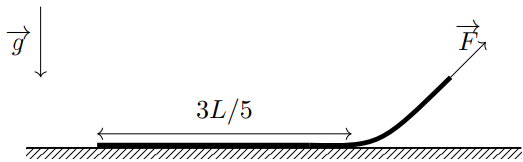
\includegraphics[width=0.5\textwidth]{Figures/Problems/Fig 3.1.png}
  \begin{center}
    \figurename{ 3.1}
  \end{center}
\end{figure}
\vspace{-0.5cm}
\noindent Xác định hệ số ma sát $\mu$ giữa sợi dây và mặt bàn để trạng thái cân bằng này có thể xảy ra.

\subsubsection*{Phần B: Quay đầu}
\noindent Alice đặt sợi dây lên mặt đất và bắt đầu kéo một đầu của dây về hướng đầu còn lại với vận tốc không đổi $v$. Trong trường hợp này, hệ số ma sát giữa dây và mặt đất là rất lớn. Bỏ qua mọi ảnh hưởng tại điểm mà sợi dây bị uốn cong.
\begin{figure}[H]
  \centering
  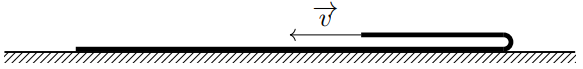
\includegraphics[width=0.5\textwidth]{Figures/Problems/Fig 3.2.png}
  \begin{center}
    \figurename{ 3.2}
  \end{center}
\end{figure}
\vspace{-0.5cm}
\noindent Lực tối thiểu mà Alice cần tác dụng lên sợi dây là bao nhiêu?

\subsubsection*{Phần C: Trượt khỏi bàn}
\noindent Alice để sợi dây trên một cái bàn có độ cao $h > L$ với một đoạn dây có chiều dài $l_0 < L$ buông ra ngoài mép bàn. Tại thời điểm $t = 0$, sợi dây đang đứng yên. Giả sử $l_0$ đủ dài để sợi dây bắt đầu trượt xuống khỏi bàn. Hệ số ma sát giữa bàn và sợi dây là $\mu$. Bỏ qua mọi ảnh hưởng tại điểm cong của sợi dây. Gia tốc trọng trường là $\vec{g}$.
\begin{figure}[H]
  \centering
  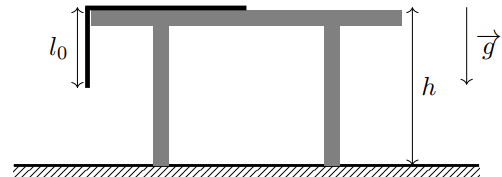
\includegraphics[width=0.5\textwidth]{Figures/Problems/Fig 3.3.png}
  \begin{center}
    \figurename{ 3.3}
  \end{center}
\end{figure}
\vspace{-0.5cm}

\begin{enumerate}
  \item Tìm vận tốc của sợi dây ngay tại thời điểm toàn bộ sợi dây đã rời khỏi bàn.
  \item Lập phương trình vi phân mô tả chiều dài đoạn dây buông ra ngoài bàn.
  \item Giải phương trình vi phân trên với giả thiết sau:
        \begin{equation*}
          x(t) = A \cosh \omega t + B
        \end{equation*}
        Với $A$ và $B$ là các hằng số cần xác định.
\end{enumerate}
\noindent\textit{Gợi ý:}
\begin{equation*}
  \cosh t = \frac{e^t + e^{-t}}{2}
\end{equation*}

\subsubsection*{Phần D: Treo vật}
\noindent Alice sử dụng một chiếc bàn nhỏ hơn và buộc hai quả nặng có khối lượng $m$ vào hai đầu của sợi dây. Quả nặng bên trái chỉ có thể di chuyển lên xuống, trong khi quả nặng bên phải có thể di chuyển cả lên xuống và sang trái phải. Tại thời điểm $t = 0$, hệ đang đứng yên với góc lệch $\theta = \varepsilon \ll 1$. Gia tốc trọng trường là $\vec{g}$.
\begin{figure}[H]
  \centering
  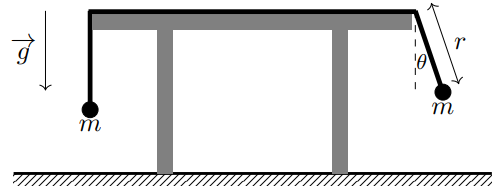
\includegraphics[width=0.5\textwidth]{Figures/Problems/Fig 3.4.png}
  \begin{center}
    \figurename{ 3.4}
  \end{center}
\end{figure}
\vspace{-0.5cm}
\noindent Tìm gia tốc trung bình của quả nặng bên trái. Giả sử $\dot{r} \approx 0$.

\noindent\textit{Gợi ý}: Với $x \ll 1$, ta có:
\begin{equation*}
  \cos x \approx 1 - \frac{1}{2}x^2
\end{equation*}
\begin{equation*}
  \int_0^{2\pi} \cos^2 t \, dt = \int_0^{2\pi} \sin^2 t \, dt = \pi
\end{equation*}
Trong hệ tọa độ cực $(r, \theta)$, gia tốc có thể được viết dưới dạng:
\begin{equation*}
  \vec{a} = \left(r\ddot{\theta} + 2\dot{r}\dot{\theta}\right)\vec{u}_\theta + \left(\ddot{r} - r\dot{\theta}^2\right)\vec{u}_r
\end{equation*}
\noindent Trong đó $\vec{u}_\theta$ là vector đơn vị của tọa độ góc và $\vec{u}_r$ là vector đơn vị của tọa độ khoảng cách.